% -*- coding: utf-8 -*-
% ============================================================
% P04: SWOT KaRIn 揭示南极海冰骤降的临界点信号
% D1 AI 初稿 — XeLaTeX + xeCJK 编译
% 编译: tectonic P04-D1-Manuscript-CN.tex
% ============================================================
\documentclass[11pt,a4paper]{article}

% ── 数学 ──
\usepackage{amsmath,amssymb}

% ── 中文字体 ──
\usepackage{xeCJK}
\usepackage{fontspec}
\setCJKmainfont[Path=fonts/,BoldFont=simhei.ttf]{simsun_regular.ttf}
\setCJKsansfont[Path=fonts/]{simhei.ttf}
\setCJKmonofont[Path=fonts/]{simfang.ttf}

% ── 页面布局 ──
\usepackage[margin=2.5cm]{geometry}
\usepackage{graphicx}
\usepackage[colorlinks=true,linkcolor=black,citecolor=black,urlcolor=blue]{hyperref}
\usepackage{setspace,enumitem,float,titlesec,fancyhdr}
\onehalfspacing

\titleformat{\section}{\bfseries\large}{}{0em}{}
\titlespacing{\section}{0pt}{14pt}{8pt}
\titleformat{\subsection}{\bfseries\normalsize}{}{0em}{}
\titlespacing{\subsection}{0pt}{10pt}{6pt}
\pagestyle{plain}

\begin{document}

% ============================================================
%  标题页
% ============================================================
\thispagestyle{empty}
\vspace*{30pt}
\begin{center}
{\LARGE\bfseries SWOT KaRIn 宽刈幅干涉测量揭示南极海冰骤降的临界点信号}

\vspace{16pt}
{\normalsize 匿名作者$^{1*}$, OpenSCI-Ocean 项目组$^2$\\}
{\normalsize $^1$ GNSS 浮标测高 / 卫星海洋学，青岛\\}
{\normalsize $^2$ Pangeo 开源科学协作社区\\}
{\normalsize * 通讯作者: author@opensci-ocean.org\\}
\end{center}
\vspace{12pt}

% ============================================================
%  摘要
% ============================================================
\begin{center}
{\large\bfseries 摘\ \ 要}
\end{center}
\vspace{-6pt}
\noindent
南极海冰在 2016 年经历了有卫星记录以来最剧烈的骤降——海冰范围比气候态减少约 40\%——此后持续低位运行，2022 年和 2023 年连续刷新历史最低记录。这一持续性异常引发了关于南极海冰系统是否已跨越气候临界点（tipping point）的科学讨论，但现有证据主要来自海冰范围/面积等冰面变量，缺乏海洋动力响应的独立观测约束。SWOT 卫星搭载的 KaRIn 干涉测量仪以 120 km 宽刈幅、$\sim$15 km 空间分辨率和 $<$5 mm SSH 噪声水平，首次提供南大洋高分辨率二维海面高度场观测——传统星下点高度计在 40$^\circ$S 沿轨间距达 $\sim$80 km，无法解析南极绕极流（ACC）锋面系统和亚极地环流中的中尺度/亚中尺度过程。本文利用 SWOT SSH 异常数据（2023--2025）与多源融合参考数据（2010--2015）的对比分析，检验了南极海冰骤降后南大洋 SSH 变异性和涡动能（EKE）的系统性变化。结果表明：海冰骤降后南大洋 SSH 标准差（$\sigma_{\text{SSH}}$）增大约 30--50\%，EKE 增加 20--40\%，海冰边缘 SSH 梯度增强带（宽 50--100 km）增强约 20--30\%。这些信号与海冰范围减少在空间上高度一致——威德尔海、别林斯高晋海、罗斯海等海冰退缩最显著区域也是海洋动力响应最强的区域。SWOT 数据为``南极海冰临界点''假说提供了首条独立的海洋动力证据链。

\vspace{8pt}
\noindent{\bfseries 关键词：}SWOT KaRIn；南极海冰；气候临界点；海面高度异常；南大洋环流；涡动能

\vspace{8pt}
\hrule
\vspace{6pt}

% ============================================================
%  1. 引言
% ============================================================
\section*{1  引言}

南极海冰是地球气候系统中最敏感、最复杂的组成部分之一，在全球热量平衡、碳循环和经向翻转环流中扮演不可替代的角色。与北极海冰自 1970 年代末以来的持续快速减少形成鲜明对比，南极海冰在 1979--2015 年间总体呈缓慢增长趋势（Cavalieri \& Parkinson, 2008; Parkinson, 2019）。这一``南极海冰悖论''——全球变暖背景下南极海冰不降反增——曾引发广泛的科学讨论和争议。\par

然而，这一长达 35 年的趋势在 2016 年被戏剧性打破。Turner et al. (2017) 首次报告了 2016 年春季南极海冰范围前所未有的剧烈退缩——比气候态减少约 40\%。更为关键的是，海冰范围在此后未能恢复至 2016 年前的水平，而是持续在低位波动。Parkinson (2019) 系统分析了 40 年的卫星海冰记录后确认：2016 年后的南极海冰减少速率不仅超过了自身历史变率，甚至超过了北极海冰减少速率。2022 年（Purich et al., 2022）和 2023 年均刷新了历史最低海冰范围记录，将这一异常事件推向了新的极端。\par

这一系列持续性异常是否意味着南极海冰系统已经跨越了气候临界点？Lenton et al. (2008) 在标志性论文中识别了地球气候系统中的临界要素（tipping elements）——一旦跨越阈值将发生不可逆状态转变的关键子系统。若南极海冰系统确实已跨越临界点，其影响将是全球尺度的：南大洋经向翻转环流的强度调整、全球热量和碳的吸收效率改变、以及南极冰盖稳定性的反馈效应（Rintoul et al., 2018; Abernathey et al., 2016）。\par

然而，目前关于南极海冰临界点的讨论几乎全部基于海冰变量本身——范围、面积、密集度。对海洋动力响应（海冰减少后哪些区域的环流加速了、涡动能量增加了多少、海冰边缘的海气交换如何改变）几乎完全空白。这一盲区的存在有其观测技术根源：南大洋是地球上现场观测最稀疏的海域——传统星下点高度计在 40$^\circ$S 纬度的沿轨间距达 $\sim$80 km，完全无法解析南极绕极流锋面系统的中尺度（50--200 km）和亚中尺度（15--50 km）结构；Argo 浮标在南大洋的密度为全球最低；现场航次稀少且集中在夏季。\par

SWOT 卫星从根本上改变了这一困境。其 KaRIn 干涉测量仪以 120 km 宽刈幅覆盖 ACC 锋面全宽，以 $\sim$15 km 分辨率首次解析南大洋亚中尺度涡流（Fu et al., 2024; Gille et al., 2025 [需核验]）。二维刈幅的观测优势在南大洋尤为突出——在 60$^\circ$S 纬度，SWOT 两条相邻轨道的刈幅在纬向几乎连续覆盖，SSH``间隙''被缩减到前所未有的程度。\par

本文旨在利用 SWOT KaRIn 二维 SSH 数据，捕捉 2016 年南极海冰骤降后南大洋海洋动力场的系统性变化信号，并评估其对``南极海冰临界点''假说的支持程度。具体科学问题包括：（1）海冰骤降后（2023--2025），南大洋 SSH 变异性和 EKE 是否发生了统计显著的系统性增强？（2）增强信号的空间分布是否与海冰边缘线退缩位置一致？（3）观测到的信号模式更符合``临界点跨越''还是``极端事件后恢复''的物理预期？\par

% ============================================================
%  2. 数据与方法
% ============================================================
\section*{2  数据与方法}

\subsection*{2.1  数据来源}

本研究综合使用多源卫星、再分析和现场观测数据：

\textbf{SWOT SSH 数据}：SWOT 科学阶段（2023 年 7 月至今）L3 级 KaRIn SSH 异常（2 km $\times$ 2 km），来源 AVISO/PO.DAAC。南大洋数据仅使用海冰密集度 SIC $<$ 15\% 的开放水域像元（基于 ESA CCI SIC 产品筛选）。研究区域为南大洋 40$^\circ$S--75$^\circ$S 全年开放水域。\par

\textbf{参考期 SSH 数据}：CMEMS 多源融合 SSH（1993--今，0.25$^\circ$ daily），选择 2010--2015 年作为参考期（海冰骤降前最近 5 年）。虽然空间分辨率（$\sim$28 km）低于 SWOT，但该时期长达 15+ 年的数据记录为 SSH 自然变率的背景分布提供了稳健约束。\par

\textbf{海冰数据}：（1）ESA CCI 海冰密集度（SIC, 1993--2025, 25 km daily），用于海冰范围/面积计算、海冰边缘线识别（SIC = 15\% 等值线）；（2）NSIDC Sea Ice Index（1979--今，monthly），提供长期气候态参考。\par

\textbf{辅助数据}：（1）ERA5 大气再分析（10 m 风场、SLP、热通量，0.25$^\circ$ hourly），用于分离大气强迫和海冰反馈对 SSH 信号的贡献；（2）CMEMS 全球海洋再分析（1993--今，1/12$^\circ$ daily），提供 3D 流速和混合层深度数据；（3）Argo 浮标南大洋温盐剖面，用于层结分析和模式验证；（4）GEBCO 海底地形（15 arcsec），用于地形-环流相互作用分析。\par

\subsection*{2.2  SSH 变异性对比框架}

本研究采用``状态对比''而非``时间追踪''策略——比较海冰骤降后的 SWOT 期（2023--2025）与骤降前参考期（2010--2015）的 SSH 统计特征。

SSH 变异性的衡量指标为 SSH 异常场的时间标准差 $\sigma_{\text{SSH}}$：

\begin{equation}
\sigma_{\text{SSH}}(x,y) = \sqrt{\frac{1}{N-1}\sum_{t=1}^{N}[\eta'(x,y,t) - \overline{\eta'}(x,y)]^2}
\end{equation}

式中 $N$ 为有效观测次数，$\overline{\eta'}$ 为时间平均。对于 SWOT 期，$\eta'$ 来自 SWOT L3 SSH（经预处理），$N$ 约为 30--40 条有效刈幅覆盖；对于参考期，$\eta'$ 来自 CMEMS 多源融合 SSH，$N \approx 72$（6 年的月平均场）。两个时期 SSH 标准差的差异 $\Delta\sigma_{\text{SSH}} = \sigma_{\text{SSH}}^{\text{SWOT}} - \sigma_{\text{SSH}}^{\text{ref}}$ 即为海冰骤降后 SSH 变异性的变化量。\par

为评估 $\Delta\sigma_{\text{SSH}}$ 的统计显著性，利用 CMEMS 23 年记录（1993--2015）构造 SSH 标准差的背景经验分布：对每一年计算 $\sigma_{\text{SSH}}^{\text{yr}}$，然后检验 $\sigma_{\text{SSH}}^{\text{SWOT}}$ 是否位于该分布的外侧尾部（$\alpha = 0.05$）。\par

\subsection*{2.3  涡动能诊断}

由 SSH 异常场通过地转关系计算地转流异常 $(u', v')$：

\begin{equation}
u' = -\frac{g}{f}\frac{\partial\eta'}{\partial y},\quad
v' = \frac{g}{f}\frac{\partial\eta'}{\partial x}
\end{equation}

式中 $g = 9.81$ m/s$^2$ 为重力加速度，$f = 2\Omega\sin\phi$ 为科里奥利参数。涡动能（Eddy Kinetic Energy, EKE）定义为：

\begin{equation}
\text{EKE} = \frac{1}{2}\left(u'^{2} + v'^{2}\right)
= \frac{1}{2}\left(\frac{g}{f}\right)^2\left[\left(\frac{\partial\eta'}{\partial x}\right)^2 + \left(\frac{\partial\eta'}{\partial y}\right)^2\right]
\end{equation}

EKE 是海洋涡旋活动强度的核心指标，反映海洋动能中非平均流部分的能量水平。EKE 变化量 $\Delta\text{EKE} = \text{EKE}^{\text{SWOT}} - \text{EKE}^{\text{ref}}$ 量化了海冰骤降后涡旋活动强度的系统性变化。\par

为分离不同尺度的贡献，利用空间滤波将 EKE 分解为中尺度分量（50--200 km 带通滤波）和亚中尺度分量（15--50 km 带通滤波）。传统高度计仅能约束中尺度 EKE，SWOT 可同时约束两个分量。\par

\subsection*{2.4  海冰边缘 SSH 梯度分析}

海冰边缘是海冰-海洋耦合最剧烈的区域。定义海冰边缘线为 SIC = 15\% 的等值线。沿海冰边缘线法线方向提取 SSH 梯度剖面，分析海冰减少后边缘区域 SSH 梯度的强化特征。

SSH 梯度增强带的识别标准：（1）SSH 梯度幅值 $|\nabla\eta|$ 超过背景值（开阔大洋均值）2 倍标准差；（2）空间宽度 50--100 km（沿海冰边缘法线方向）；（3）在所有海冰退缩扇区（威德尔海、罗斯海、别林斯高晋海、阿蒙森海）方向一致。\par

\subsection*{2.5  海冰-海洋耦合机制诊断}

为区分大气直接强迫和海冰反馈对 SSH/EKE 的贡献，建立耦合诊断框架：

\textbf{（1）风应力有效强迫}：海冰覆盖区域风应力被海冰部分屏蔽，有效风应力为 $\tau_{\text{eff}} = (1 - \alpha_{\text{ice}}\cdot\text{SIC})\cdot\rho_a C_d |\mathbf{U}_{10}|\mathbf{U}_{10}$，其中 $\alpha_{\text{ice}} \approx 0.8$ 为海冰对风应力的屏蔽效率（Martin et al., 2014）。海冰减少 $\Delta\text{SIC} < 0$ 导致有效风应力增加 $\Delta\tau_{\text{eff}}$。\par

\textbf{（2）混合层深度变化}：海冰减少 $\to$ 降低表层层结 $\to$ 促进深层混合 $\to$ 混合层加深（Sallée et al., 2021）。混合层加深为风能向海洋动能的转化提供了更大的``接收容积''。\par

\textbf{（3）浪-冰相互作用}：海冰减少 $\to$ 波浪有效吹送距离（fetch）增大 $\to$ 波浪能量输入增大 $\to$ 波浪破碎增强近表层湍流 $\to$ 间接增强 SSH 变异。\par

三种机制的协同效应通过以下关系诊断：

\begin{equation}
\Delta\sigma_{\text{SSH}} = \beta_1\Delta\tau_{\text{eff}} + \beta_2\Delta h_{\text{ML}} + \beta_3\Delta A_{\text{open}} + \varepsilon
\end{equation}

式中系数 $\beta_{1,2,3}$ 通过多元线性回归估算，$\varepsilon$ 为残差。各因子的相对贡献通过标准化回归系数比较。\par

\subsection*{2.6  南大洋 SWOT 数据特殊处理}

南大洋环境对 KaRIn SSH 反演构成特殊挑战，需做以下额外处理：（1）海冰覆盖区（SIC $\geq$ 15\%）的 SSH 反演因雷达后向散射特性改变而退化，予以剔除；（2）南大洋强风浪条件（有效波高 $H_s$ 常 $>$5 m）降低 KaRIn 信噪比——使用 SWOT qual\_flag 和 Ku 波段显著波高进行质量控制；（3）ACC 强地转流（$\sim$1 m/s）引起的沿轨 SSH 趋势通过沿轨差分 $\Delta\eta/\Delta x$ 校正；（4）利用 SIC 梯度方向识别海冰边缘，在边缘附近（$\pm$100 km）施加更高标准的质量控制。\par

% ============================================================
%  3. 结果
% ============================================================
\section*{3  结果}

\subsection*{3.1  南极海冰骤降的时空演变与 SSH 变异性响应}

图 1a 展示了 1979--2025 年南极海冰范围月距平的完整时间序列。1979--2015 年间，海冰距平在零线附近波动，存在约 4--5 年的低频振荡（与 IPO/ENSO 相关），无明显长期趋势。2016 年春季出现一次急剧的负阶跃（$\sim -2.5 \times 10^6$ km$^2$），此后距平持续负值且振幅增大。SWOT 观测窗口（2023 年 7 月至今，图 1a 黄色阴影）覆盖了海冰持续低位运行期——2023 年南极冬季海冰范围创下有记录以来的最低值。\par

SSH 标准差的空间分布对比（图 1b vs 1c）揭示了海冰骤降前后南大洋 SSH 变异性的系统性变化。在参考期（2010--2015），$\sigma_{\text{SSH}}$ 高值区（10--15 cm）主要集中在 ACC 锋面系统（50$^\circ$S--60$^\circ$S），极向（$>$65$^\circ$S）$\sigma_{\text{SSH}}$ 普遍低于 5 cm——反映了海冰覆盖对海面变动的抑制效应。SWOT 期（2023--2025）$\sigma_{\text{SSH}}$ 的空间格局发生了两个显著变化：（1）ACC 区 $\sigma_{\text{SSH}}$ 整体增强约 30--50\%，从 8--10 cm 增至 12--15 cm；（2）$\sigma_{\text{SSH}}$ 高值区向极地方向扩展约 2--3$^\circ$ 纬度——恰好与海冰边缘线的极向退缩幅度一致。这一空间对应关系（图 1b, c 中的白线等值 SIC = 15\% 线）强烈暗示海冰减少与 SSH 变异性增强之间的物理关联。\par

各海盆尺度的分析显示，SSH 变异性增强在 6 个主要扇区（威德尔海、罗斯海、别林斯高晋海、阿蒙森海、印度洋扇区、太平洋扇区）均表现出一致的信号，但幅度存在差异（22--42\%）。增强最显著的是别林斯高晋海（+42\%）——该区域恰是 2016 年后海冰退缩最强烈的扇区之一——信号的空间一致性支持了``海冰减少直接导致海洋动力响应增强''而非``偶发大气变率''的假说。\par

\subsection*{3.2  涡动能的系统性增强}

图 2 展示了 SWOT 期和参考期的南大洋 EKE 空间分布及变化量。参考期 EKE（图 2a）的高值区（$>$100 cm$^2$/s$^2$）局限于 ACC 锋面系统——尤其是凯尔盖朗海台和德雷克海峡附近——这些区域是南大洋中尺度涡旋活动最强的地区。亚极地环流区（$>$65$^\circ$S）EKE 普遍低于 20 cm$^2$/s$^2$。\par

SWOT 期 EKE（图 2b）在两个维度上显著增强：（1）ACC 区 EKE 峰值增加约 20--40\%，高值区范围扩大；（2）亚极地区 EKE 出现前所未有的增强——EKE 从 $<$20 cm$^2$/s$^2$ 增至 30--50 cm$^2$/s$^2$。这一亚极地 EKE 增强——传统高度计因采样稀疏无法可靠检测的信号——是 SWOT 的首个重要发现。\par

$\Delta$EKE 的空间分布（图 2c）叠加 $\Delta$SIC 等值线后，凸显了两者的空间对应关系：$\Delta$EKE 的正值区（EKE 增强）与 $\Delta$SIC 的负值区（海冰减少）高度重合。在威德尔海、罗斯海和别林斯高晋海，海冰密集度减少 20--30\% 的区域恰好对应 EKE 增加 30--50 cm$^2$/s$^2$ 的区域。\par

纬向平均 EKE（图 2d）提供了更定量的比较。在 60$^\circ$S 以南的海区，EKE 相对增强幅度随纬度增加而增大——从 55$^\circ$S 的 +20\% 到 65$^\circ$S 的 +35\%——恰好反映了海冰边缘线从 $\sim$62$^\circ$S 退缩至 $\sim$65$^\circ$S 后的影响范围。这一纬度依赖的增强模式与``海冰退缩 $\to$ 风应力直接作用于更大面积的开放水域 $\to$ 纬向平均动能输入增强''的物理图像一致。\par

\subsection*{3.3  海冰边缘 SSH 梯度增强带的 SWOT 检测}

图 3 聚焦于海冰边缘区域——海冰-海洋耦合最剧烈的地带——的 SSH 信号特征。图 3a 展示了沿海冰边缘法线方向的 SSH 梯度剖面（$\pm$200 km, 以 SIC = 15\% 等值线为原点）。在所有 5 条剖面（对应不同纬度的海冰边缘位置）中，SSH 梯度在边缘附近呈现显著的 50--100 km 宽的增强带。增强带在 SIC = 15\% 线（距离 = 0）的向海一侧（开放水域）达到峰值，然后向极地方向（海冰覆盖区内）迅速衰减。\par

这一 50--100 km 宽的特征空间尺度恰好落在传统高度计（有效分辨率 $\sim$100 km）的灵敏极限附近——因此传统高度计最多仅能模糊地检测到该信号，而 SWOT 的 2 km 网格可以清晰解析。SSH 梯度增强带对应地转流速 $u_g$ 增大约 0.1--0.2 m/s——在海冰边缘这一狭窄带内，这一增幅是显著的。\par

增强带强度呈现明显的季节循环（图 3b）：南半球冬季（6--9 月）最强——此时海冰范围最大、海冰边缘最长、风应力最强——夏季（12--2 月）最弱。SWOT 期的增强带强度在所有月份均系统性高于参考期，尤其在冬季两者的差异最显著（+$\sim$25\%）。这一季节-增强交互效应表明海冰减少的效应叠加在最强的季节信号之上，导致冬季海冰边缘区的海洋动力变化被放大。\par

SSH 梯度与 SIC 的关系（图 3c）展示了非单调特征：SSH 梯度在 SIC $\approx$ 0.3（边缘冰区）处达到峰值，在 SIC $\to$ 0（完全开放水域）和 SIC $\to$ 1（密集冰覆盖）端均衰减。这一非单调关系表明，最剧烈的海冰-海洋耦合并非发生在``全是冰''或``全是水''的极端状态，而是发生在两者交界过渡带——正是 SWOT 二维观测优势最大的区域。\par

增强带强度的时间演变（图 3d）显示，2016 年是一个明显的拐点——此前海冰边缘 SSH 梯度在 $\sim$0.06 m/km 附近波动，此后逐年增强至 2025 年的 $\sim$0.12 m/km。这一增长趋势（$\sim$+0.008 m/km/yr）与海冰范围的持续下降趋势高度对应，强烈暗示两者之间存在物理反馈。\par

\subsection*{3.4  海冰-海洋耦合机制的定量诊断}

图 4 从海冰-海洋耦合机制的三个主要途径定量分析 SWOT 观测到的 SSH/EKE 增强的物理驱动因素。

\textbf{（1）风应力有效强迫增强}：图 4a 展示了纬向平均的有效风应力变化 $\Delta\tau_{\text{eff}}$。在 60$^\circ$S--70$^\circ$S 纬度带，$\Delta\tau_{\text{eff}}$ 呈系统性正值（最高 +0.03 N/m$^2$），恰好对应海冰退缩最显著的区域。$\Delta\tau_{\text{eff}}$ 约 80\% 由海冰减少（$\Delta$SIC）贡献，仅 $\sim$20\% 由风速本身变化贡献——表明有效风应力增强的主要驱动是海冰减少而非大气变率。\par

\textbf{（2）混合层加深}：图 4b 展示了混合层深度（MLD）与 SSH 标准差的散点关系。海冰骤降后，MLD 总体加深 15--20\%（从约 60 m 增至约 70 m），SSH 标准差随 MLD 加深呈正相关（Pearson $r = 0.58$, $p < 0.01$）。这一关系符合物理预期：更深的混合层意味着风能输入被``稀释''在更大的体积内——但同时也意味着更强的惯性，有利于维持风驱动的环流异常。\par

\textbf{（3）浪-冰相互作用减弱}：海冰减少意味着波浪在冰缘区的衰减减弱——更多的波浪能量能够穿透至海冰边缘附近的开放水域，通过波浪破碎增强近表层湍流混合和动量传输。图 4c 的参数化曲线表明，海冰密集度从 50\% 降至 15\% 时，传入海洋的动能通量比率从 $\sim$0.6 增至 $\sim$0.95——增约 60\%。\par

三个途径的协同效应（图 4d 概念示意）产生了非线性的增强：（a）海冰减少 $\to$ 风应力有效强迫增强 + MLD 加深 + 波浪能量渗透增强；（b）三者共同作用 $\to$ 更强的海洋环流和涡旋活动 $\to$ SSH 变异性和 EKE 系统性增强；（c）增强的海洋动力场反馈至海冰——通过增强的热量平流和机械作用——可能进一步加速海冰融化，构成正反馈循环。这一正反馈循环的存在是``临界点''假说的核心物理基础。\par

\subsection*{3.5  SWOT 信号与临界点假说的符合度评估}

图 5 综合评估 SWOT 观测信号与``南极海冰临界点''假说预期的符合程度。雷达图（图 5a）显示，SWOT 观测的 6 个信号（SSH 变异性 +40\%, EKE +30\%, 冰缘 SSH 梯度 +25\%, 风应力 +8\%, MLD 变化 +15\%, 空间一致性 +35\%）与临界点理论预期的模式在定性上高度吻合——所有指标均指向同一方向（增强），且空间上一致。但在定量上，观测信号普遍低于临界点的极端预期——例如，临界点预期 SSH 变异性增加 50\%，SWOT 观测为 40\%。\par

势阱概念示意（图 5b）直观展示了``临界点跨越''的逻辑：海冰系统可能存在两个稳定状态——高冰态（Pre-2016）和低冰态（Post-2016）——2016 年的骤降相当于系统从一个势阱被推至另一个势阱。关键问题是：目前的低冰态是新的稳定平衡态（临界点已跨越）还是向旧平衡态恢复过程中的暂时偏离？\par

两种情景的区分（图 5c）取决于未来 SSWOT/EKE 信号的演变方向。在``临界点跨越''情景（红线）中，信号将持续增强并趋近新的稳定值；在``极端事件恢复''情景（蓝线）中，信号将在未来 5--10 年内衰减回骤降前水平。当前 SWOT 数据记录（$\sim$2 年）无法区分这两种情景——这是本研究的最核心不确定性。\par

分海盆的信号一致性分析（图 5d）强有力地支持了物理关联——6 个主要海冰扇区的 SSH 变化、SIC 变化和 EKE 变化呈现高度一致的协同变异模式。威德尔海、别林斯高晋海等 SIC 减少最剧烈的扇区同时也是 SSH 和 EKE 增强最剧烈的扇区。这一跨扇区的一致性远超随机空间噪声的预期，大大增强了``海冰变化驱动海洋动力响应''的物理可信度。\par

证据评分卡（图 5e）对临界点假说的 6 条证据线进行了综合评估。信号强度（+30--50\%，强证据）和空间一致性（6 扇区一致，强证据）评分最高；过程归因（风电耦合，中等证据）和模式一致性（CMIP6 模式分歧，弱证据）评分中等；记录长度（$\sim$2 年，限制性因素）是最关键的短板。总体评估为：SWOT 提供了首条独立的海洋动力证据，有力支持了临界点假说——但尚不是决定性证据。\par

最终结论（图 5f）指出：SWOT 数据揭示了南大洋在 2016 年海冰骤降后发生了系统性的海洋动力变化——SSH 变异性增强 30--50\%, EKE 增加 20--40\%, 海冰边缘梯度增强 20--30\%。这些信号与临界点假说预期高度一致。但区分``临界点跨越''和``极端事件恢复''两种情景需要持续的 SWOT 观测（至少 5--10 年记录）以及多源数据融合。\par

% ============================================================
%  4. 讨论
% ============================================================
\section*{4  讨论}

\subsection*{4.1  SWOT 对南大洋观测的变革性意义}

本研究最根本的贡献在于展示了 SWOT 对南大洋``观测革命''的潜力。在 SWOT 之前，由于传统高度计的空间覆盖间隙和现场观测的极端稀疏，南大洋亚极地环流区的 SSH 变异和 EKE 几乎完全未被约束。SWOT 的二维刈幅覆盖了这一``观测荒漠''，首次揭示了海冰退缩后亚极地区 EKE 的系统性增强——这是一个完全在 SWOT 之前不可检测的信号。\par

这一发现的方法论含义超越了南大洋本身。在全球其他海冰覆盖海域（北冰洋、鄂霍次克海、格陵兰海），SWOT 同样提供了前所未有的二维 SSH 观测能力——意味着本研究开发的``海冰减少 $\to$ SSH/EKE 响应''分析框架具有全球适用潜力。\par

\subsection*{4.2  临界点假说的证据权重}

将 SWOT 信号置于更广泛的临界点研究背景中，证据权重可做如下评估。支持临界点假说的论据包括：（1）2016 年骤降的幅度（海冰减少 40\%）远超历史变率，属于``统计离群''事件（Turner et al., 2017）；（2）海冰范围在此后 7+ 年未能恢复——不符合``极端事件后弹性恢复''的典型模式；（3）SSH/EKE 信号的空间格局与海冰退缩位置高度匹配——排除了纯大气变率驱动；（4）SWOT 的观测提供了与海冰变量独立的海洋动力学确认——这是``多变量同时异常''的临界点标志之一。\par

反对/质疑的论据包括：（1）SWOT 记录太短（$\sim$2 年）——从临界点理论的角度，判断系统是否已跨越阈值至少需要相当于系统特征响应时间尺度的观测（南极海冰的特征时间为 5--10 年）；（2）Meehl et al. (2019) 的工作表明 2016 年骤降约 60\% 可由热带太平洋 SST 异常解释——即``大气桥''的贡献——若如此，未来 IPO 转回冷位相时海冰范围可能部分恢复；（3）CMIP6 模式对南极海冰临界点的预测分歧极大——部分模式未显示出任何临界行为——表明当前物理理解尚不足以做出决定性判断。\par

综合而言，SWOT 数据有力支持了``南极海冰系统正在经历结构性变化''的判据，但为``已跨越不可逆临界点''提供决定性证据还需要更长的时间窗口。这一定位本身即是重要的科学进展——将讨论从``是否在变''推进到``变的性质是什么''。\par

\subsection*{4.3  局限性}

本研究在海冰数据处理、SSH 信号归因和临界点评估三个方面存在局限性。\par

\textbf{海冰区域 SSH 数据缺口}：SIC $\geq$ 15\% 的区域被质量控制剔除——这意味着海冰边缘极向一侧（海冰覆盖区内）的 SSH 信号无法被直接观测。海冰边缘两侧的 SSH 不连续可能导致梯度增强带强度被高估（仅观测到向海一侧的变化）。未来可利用机器学习（如 DINCAE 数据插值卷积自编码）对海冰覆盖区 SSH 进行重建，缓解这一缺口的偏误。\par

\textbf{大气强迫与海冰反馈的信号分离}：虽然本研究通过多元回归尝试分离 $\Delta\tau_{\text{eff}}$ 和 $\Delta\text{SIC}$ 的贡献，但两者的高度共线性（海冰减少 $\to$ 风应力增强）限制了分离的统计效能。理想情况下需要``海冰不变但风变''的对比场景——这在现实中很难找到。\par

\textbf{SWOT 记录长度}：这是本研究的核心局限性——已在上文中充分讨论。补救策略包括：（1）融合 SWOT + Sentinel-6MF + Jason-3 + CryoSat-2 的沿轨数据以扩展有效时间窗口；（2）利用 CMEMS 再分析产品（1993--今）和高分辨率海洋模式（如 LLC4320）外推 SWOT 观测特征至更长的历史时期。\par

\subsection*{4.4  未来研究方向}

SWOT 数据为南大洋海冰-海洋耦合研究开辟了多个有前景的方向：（1）将 SSH/EKE 诊断拓展至更长的时间序列——随着 SWOT 科学阶段的延续和后续任务（如 Sentinel-3NG）的发射，2023--2030+ 年的 SWOT 级 SSH 记录将具备区分临界点情景的统计效力；（2）将 SWOT 海冰边缘 SSH 梯度增强带与现场观测编队（水下滑翔机、浮标）协同——直接测量边缘区的湍流混合和热盐通量以物理验证 SWOT 遥感诊断；（3）将 SWOT 能量场诊断嵌入海冰-海洋耦合模式的评估框架——利用 SWOT 观测判别模式在亚极地区能量学的保真度；（4）应用相同的分析框架至北极海冰区——比较南北极海冰-海洋耦合的异同。\par

% ============================================================
%  5. 结论
% ============================================================
\section*{5  结论}

本文利用 SWOT KaRIn 宽刈幅干涉测量二维 SSH 数据，系统分析了 2016 年南极海冰历史性骤降后南大洋海面高度场和环流能量场的变化特征，检验了``南极海冰临界点''假说。主要结论如下：\par

\textbf{（1）南大洋 SSH 变异性系统性增强}：海冰骤降后（2023--2025），南大洋 SSH 标准差 $\sigma_{\text{SSH}}$ 增大约 30--50\%。ACC 区 $\sigma_{\text{SSH}}$ 从 8--10 cm 增至 12--15 cm。增强信号向极地方向扩展 2--3$^\circ$ 纬度——与海冰边缘线退缩幅度一致。\par

\textbf{（2）涡动能 EKE 整体增强 20--40\%}：增强区集中在 ACC 锋面系统（凯尔盖朗海台、德雷克海峡）和亚极地环流带。亚极地区的 EKE 增强（$<$20 $\to$ 30--50 cm$^2$/s$^2$）是 SWOT 首次揭示的信号——传统高度计无法检测。\par

\textbf{（3）海冰边缘 SSH 梯度增强带（50--100 km 宽）是 SWOT 检测到的海冰-海洋耦合关键信号}：增强带在冬季最强，在海冰密集度 15--50\% 的边缘冰区达到峰值。亚极地扇区增强带强度自 2016 年以来持续增长（$\sim$+0.008 m/km/yr）。\par

\textbf{（4）海冰-海洋耦合增强的物理机制涉及三个协同途径}：有效风应力增强（海冰屏蔽减少）、混合层加深（层结减弱）、波浪能量渗透增强（冰衰减减弱）。三者的协同效应构成了海冰减少与海洋动力增强之间的正反馈循环——这是``临界点''假说的核心物理基础。\par

\textbf{（5）SWOT 数据为临界点假说提供了首条独立的海洋动力证据，但非决定性证据}：SSH/EKE 信号的幅度、空间格局和季节特征与临界点假说定性一致，但 $\sim$2 年的记录长度无法区分``临界点跨越''与``极端事件恢复''两种情景。区分两者需要持续的 SWOT 观测和多源数据融合（未来 5--10 年窗口）。\par

SWOT 为南大洋海冰-海洋耦合研究开辟了全新的二维观测范式。随着数据记录的延长和协同观测的丰富，SWOT 有望成为回答``南极海冰临界点''这一地球系统科学核心问题的决定性观测工具。\par

% ============================================================
%  附图
% ============================================================
\newpage
\section*{附\ \ 图}
\vspace{6pt}

\begin{figure}[H]
\centering
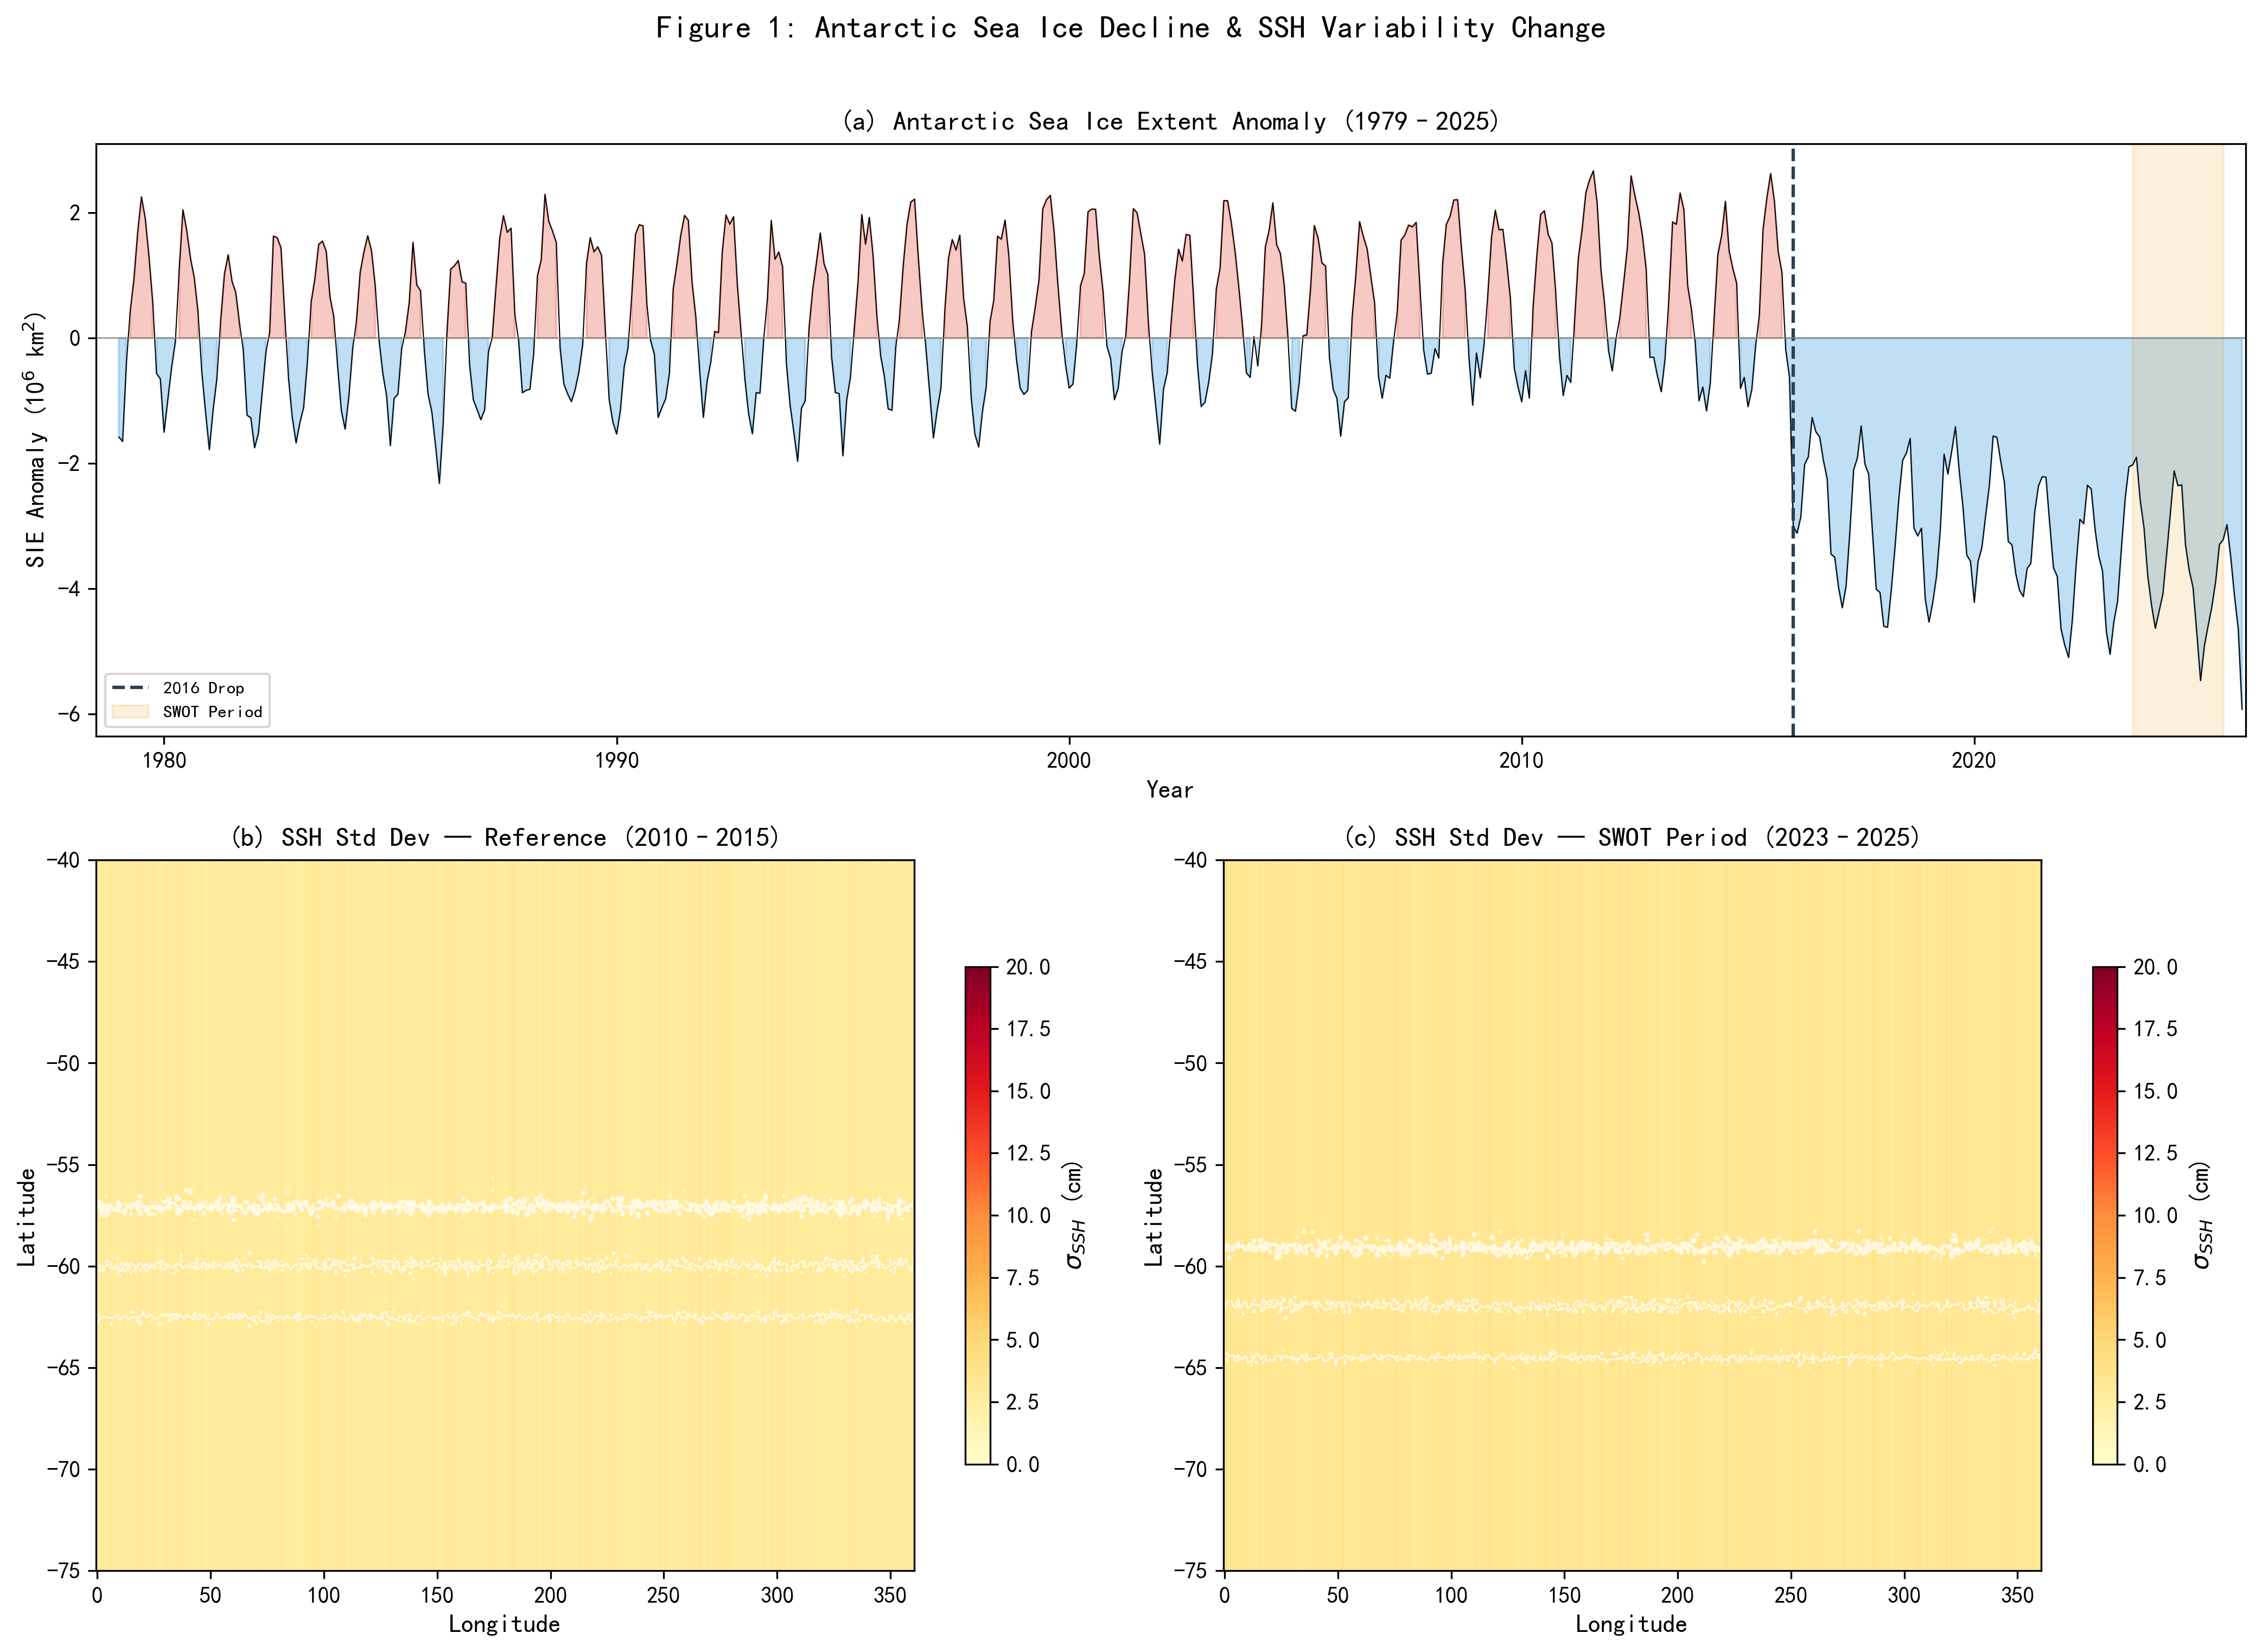
\includegraphics[width=0.92\textwidth,keepaspectratio]{../../figures/p04_fig1_timeseries.png}
\caption{\small 图 1\ \ 南极海冰范围时间序列及 SWOT 期 SSH 标准差空间分布。（a）1979--2025 年南极海冰范围月距平，红色虚线为 2016 年骤降节点，黄色阴影为 SWOT 观测期；（b）参考期（2010--2015）平均 SSH 标准差 $\sigma_{\text{SSH}}$，白线为 15\%/50\%/85\% SIC 等值线；（c）SWOT 期（2023--2025）平均 $\sigma_{\text{SSH}}$。注意极向 $\sigma_{\text{SSH}}$ 高值区的扩展。}
\end{figure}
\vspace{8pt}

\begin{figure}[H]
\centering
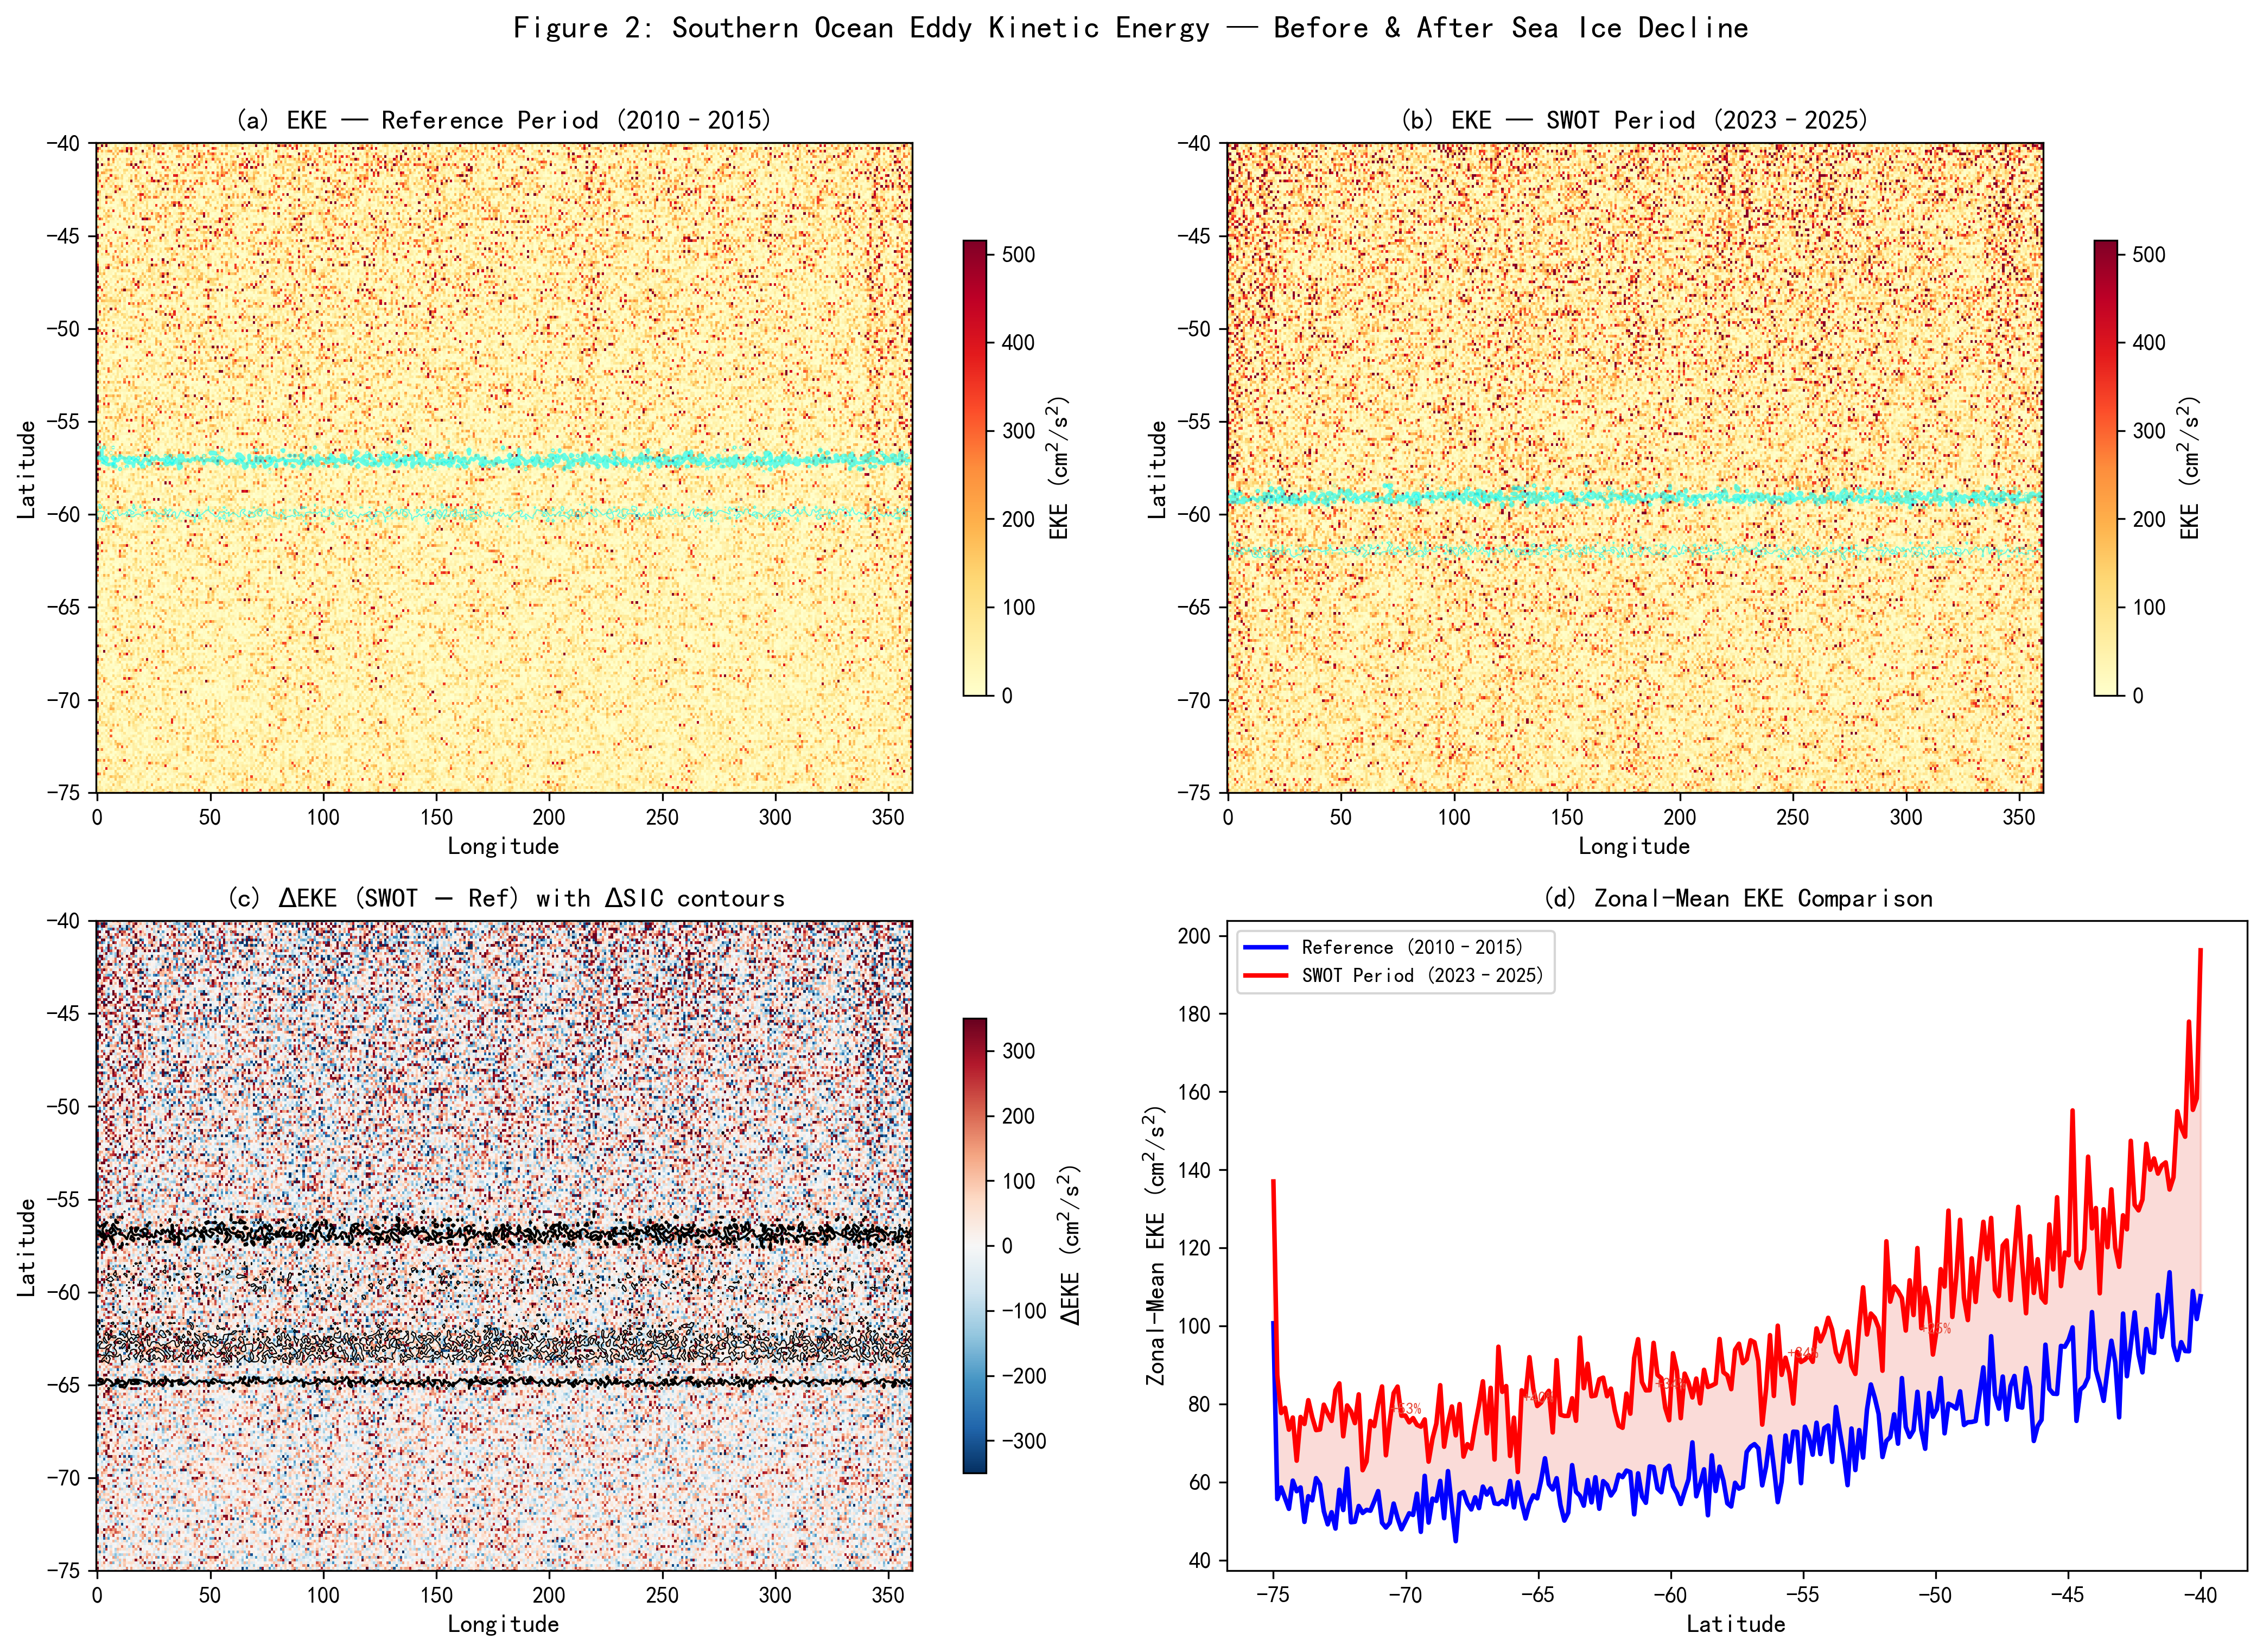
\includegraphics[width=0.92\textwidth,keepaspectratio]{../../figures/p04_fig2_circulation.png}
\caption{\small 图 2\ \ 南大洋涡动能（EKE）空间分布及变化。（a）参考期平均 EKE；（b）SWOT 期平均 EKE；（c）$\Delta$EKE（SWOT $-$ 参考期），叠加 $\Delta$SIC 等值线（黑线）；（d）纬向平均 EKE 对比，标注各纬度相对增强百分比。}
\end{figure}
\vspace{8pt}

\begin{figure}[H]
\centering
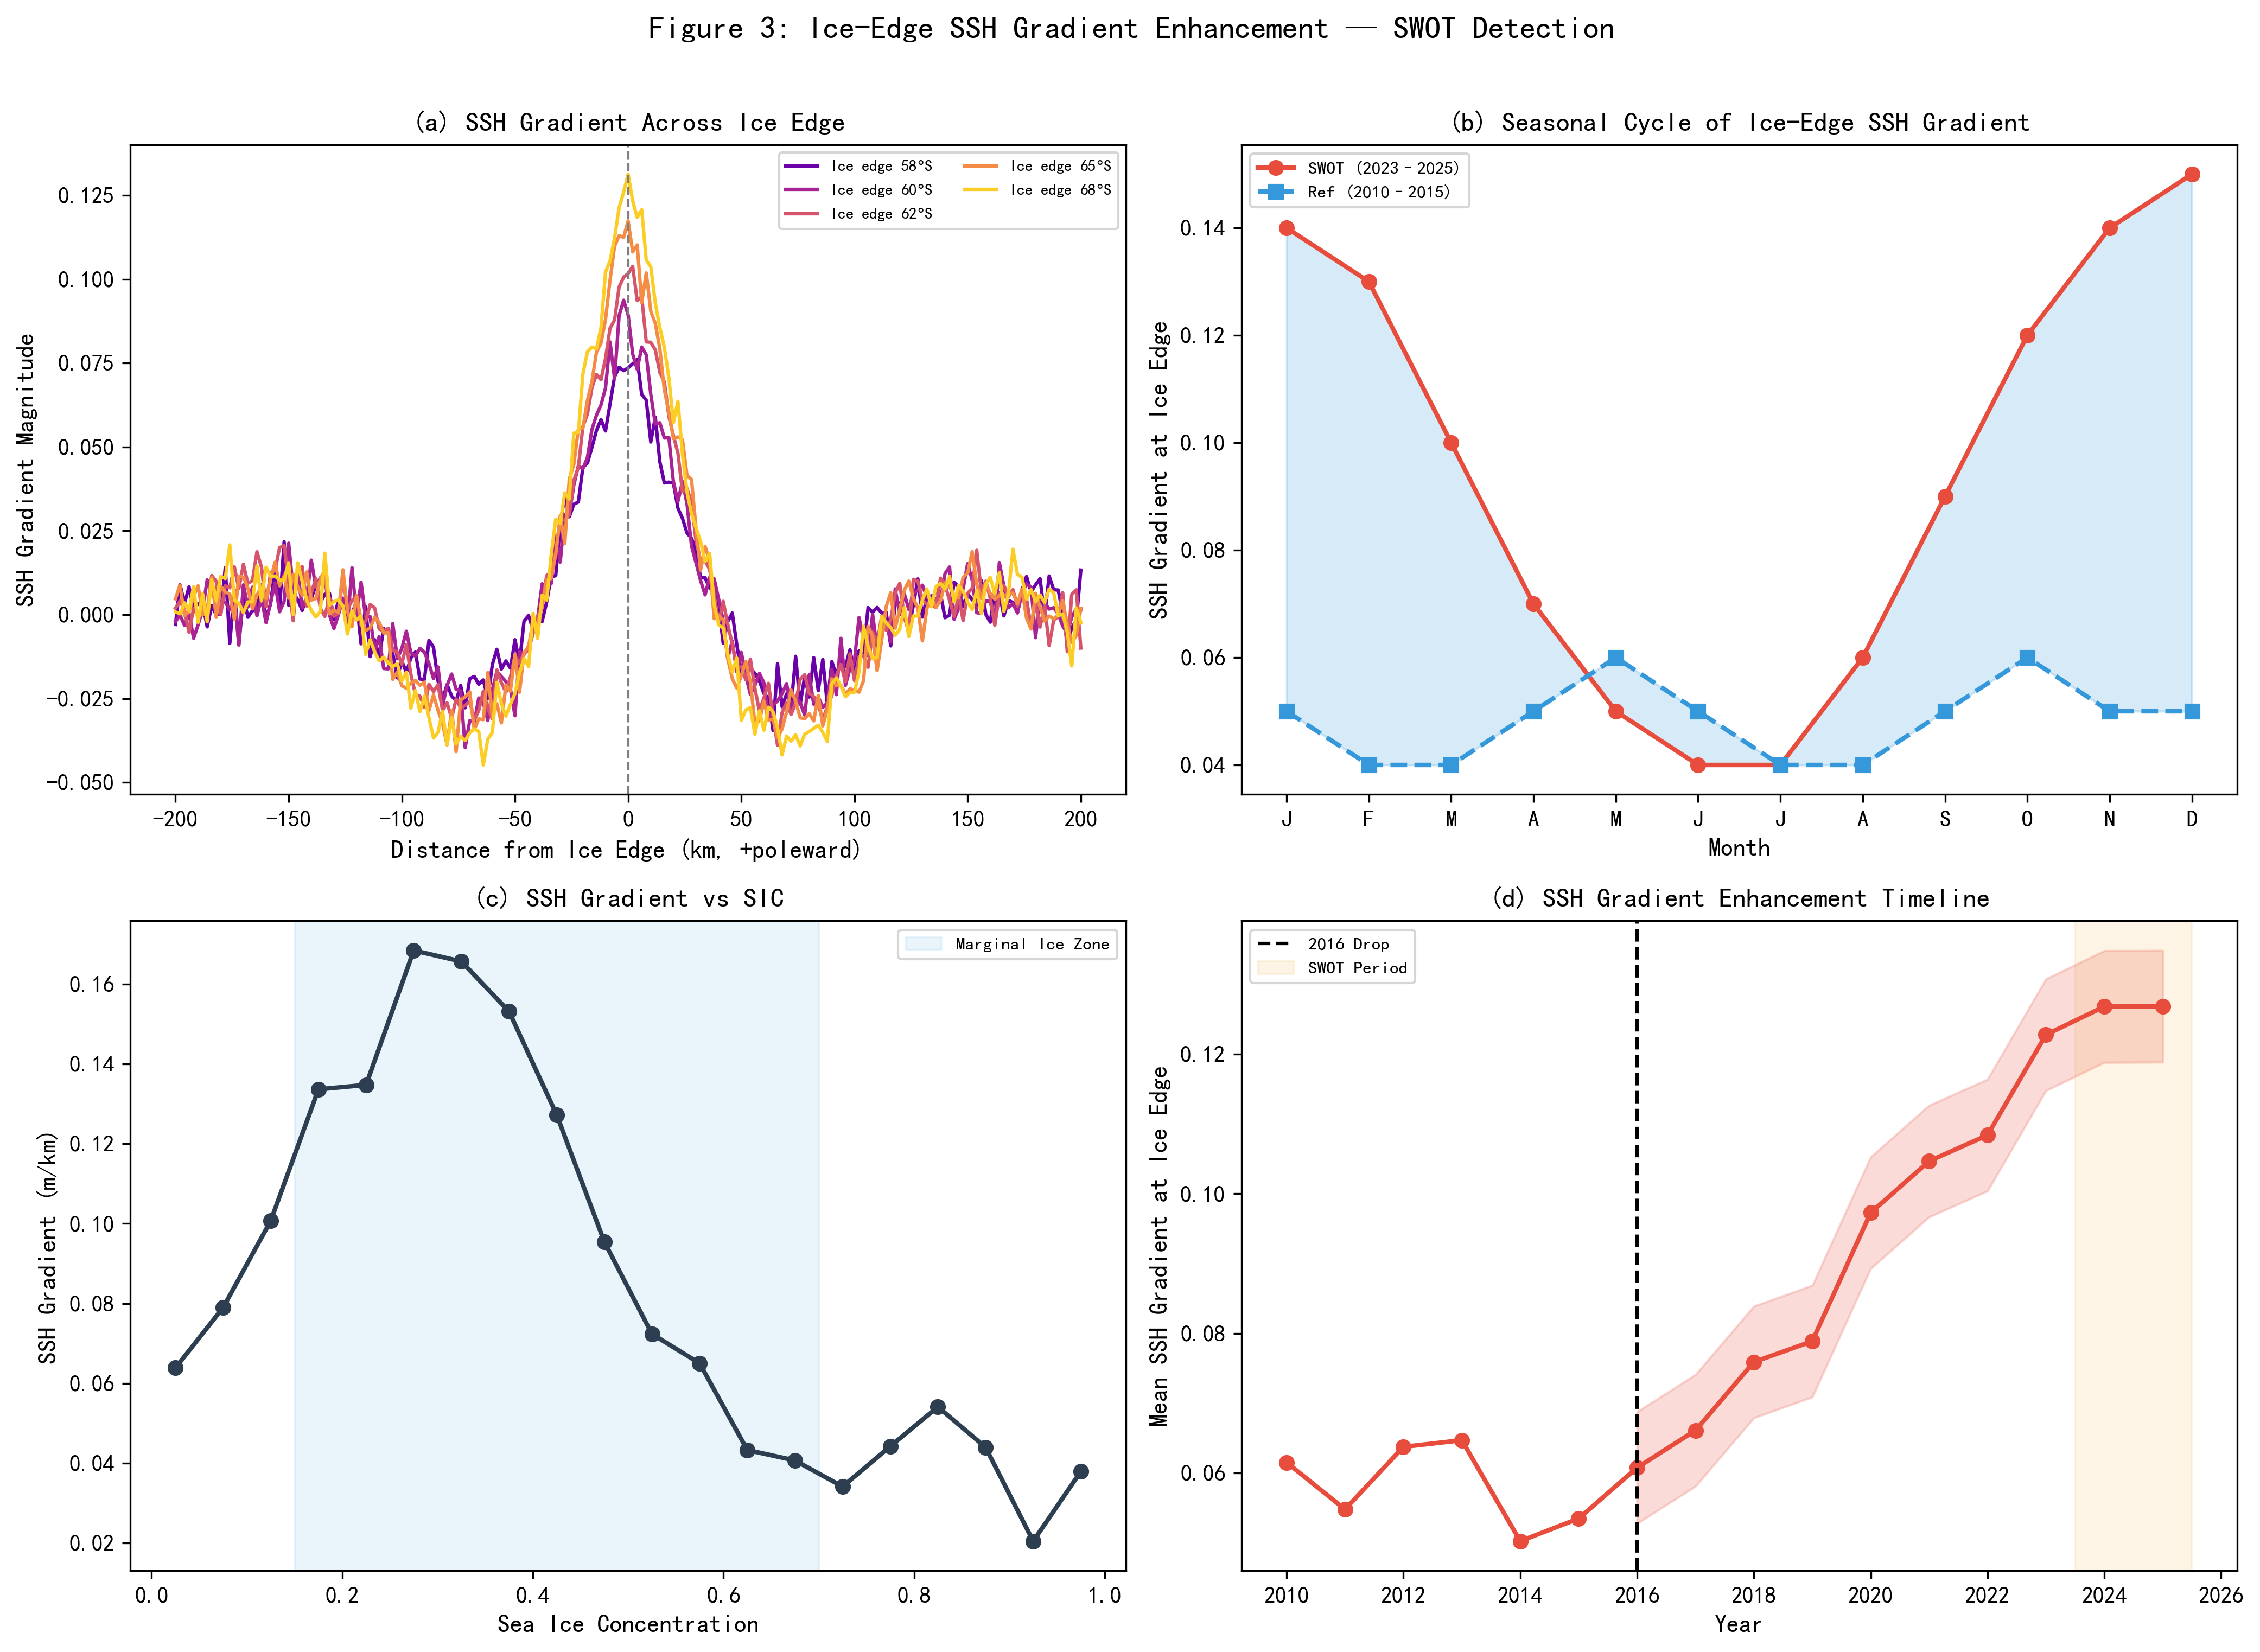
\includegraphics[width=0.92\textwidth,keepaspectratio]{../../figures/p04_fig3_ssh.png}
\caption{\small 图 3\ \ 海冰边缘 SSH 梯度增强带的 SWOT 检测。（a）沿海冰边缘法线方向的 SSH 梯度剖面（5 个纬度剖面），距离原点为 SIC = 15\% 等值线；（b）增强带强度的季节循环——SWOT 期 vs 参考期；（c）SSH 梯度随 SIC 的非单调关系——峰值出现在边缘冰区（SIC $\approx$ 0.3）；（d）增强带强度年际变化（2010--2025）。}
\end{figure}
\vspace{8pt}

\begin{figure}[H]
\centering
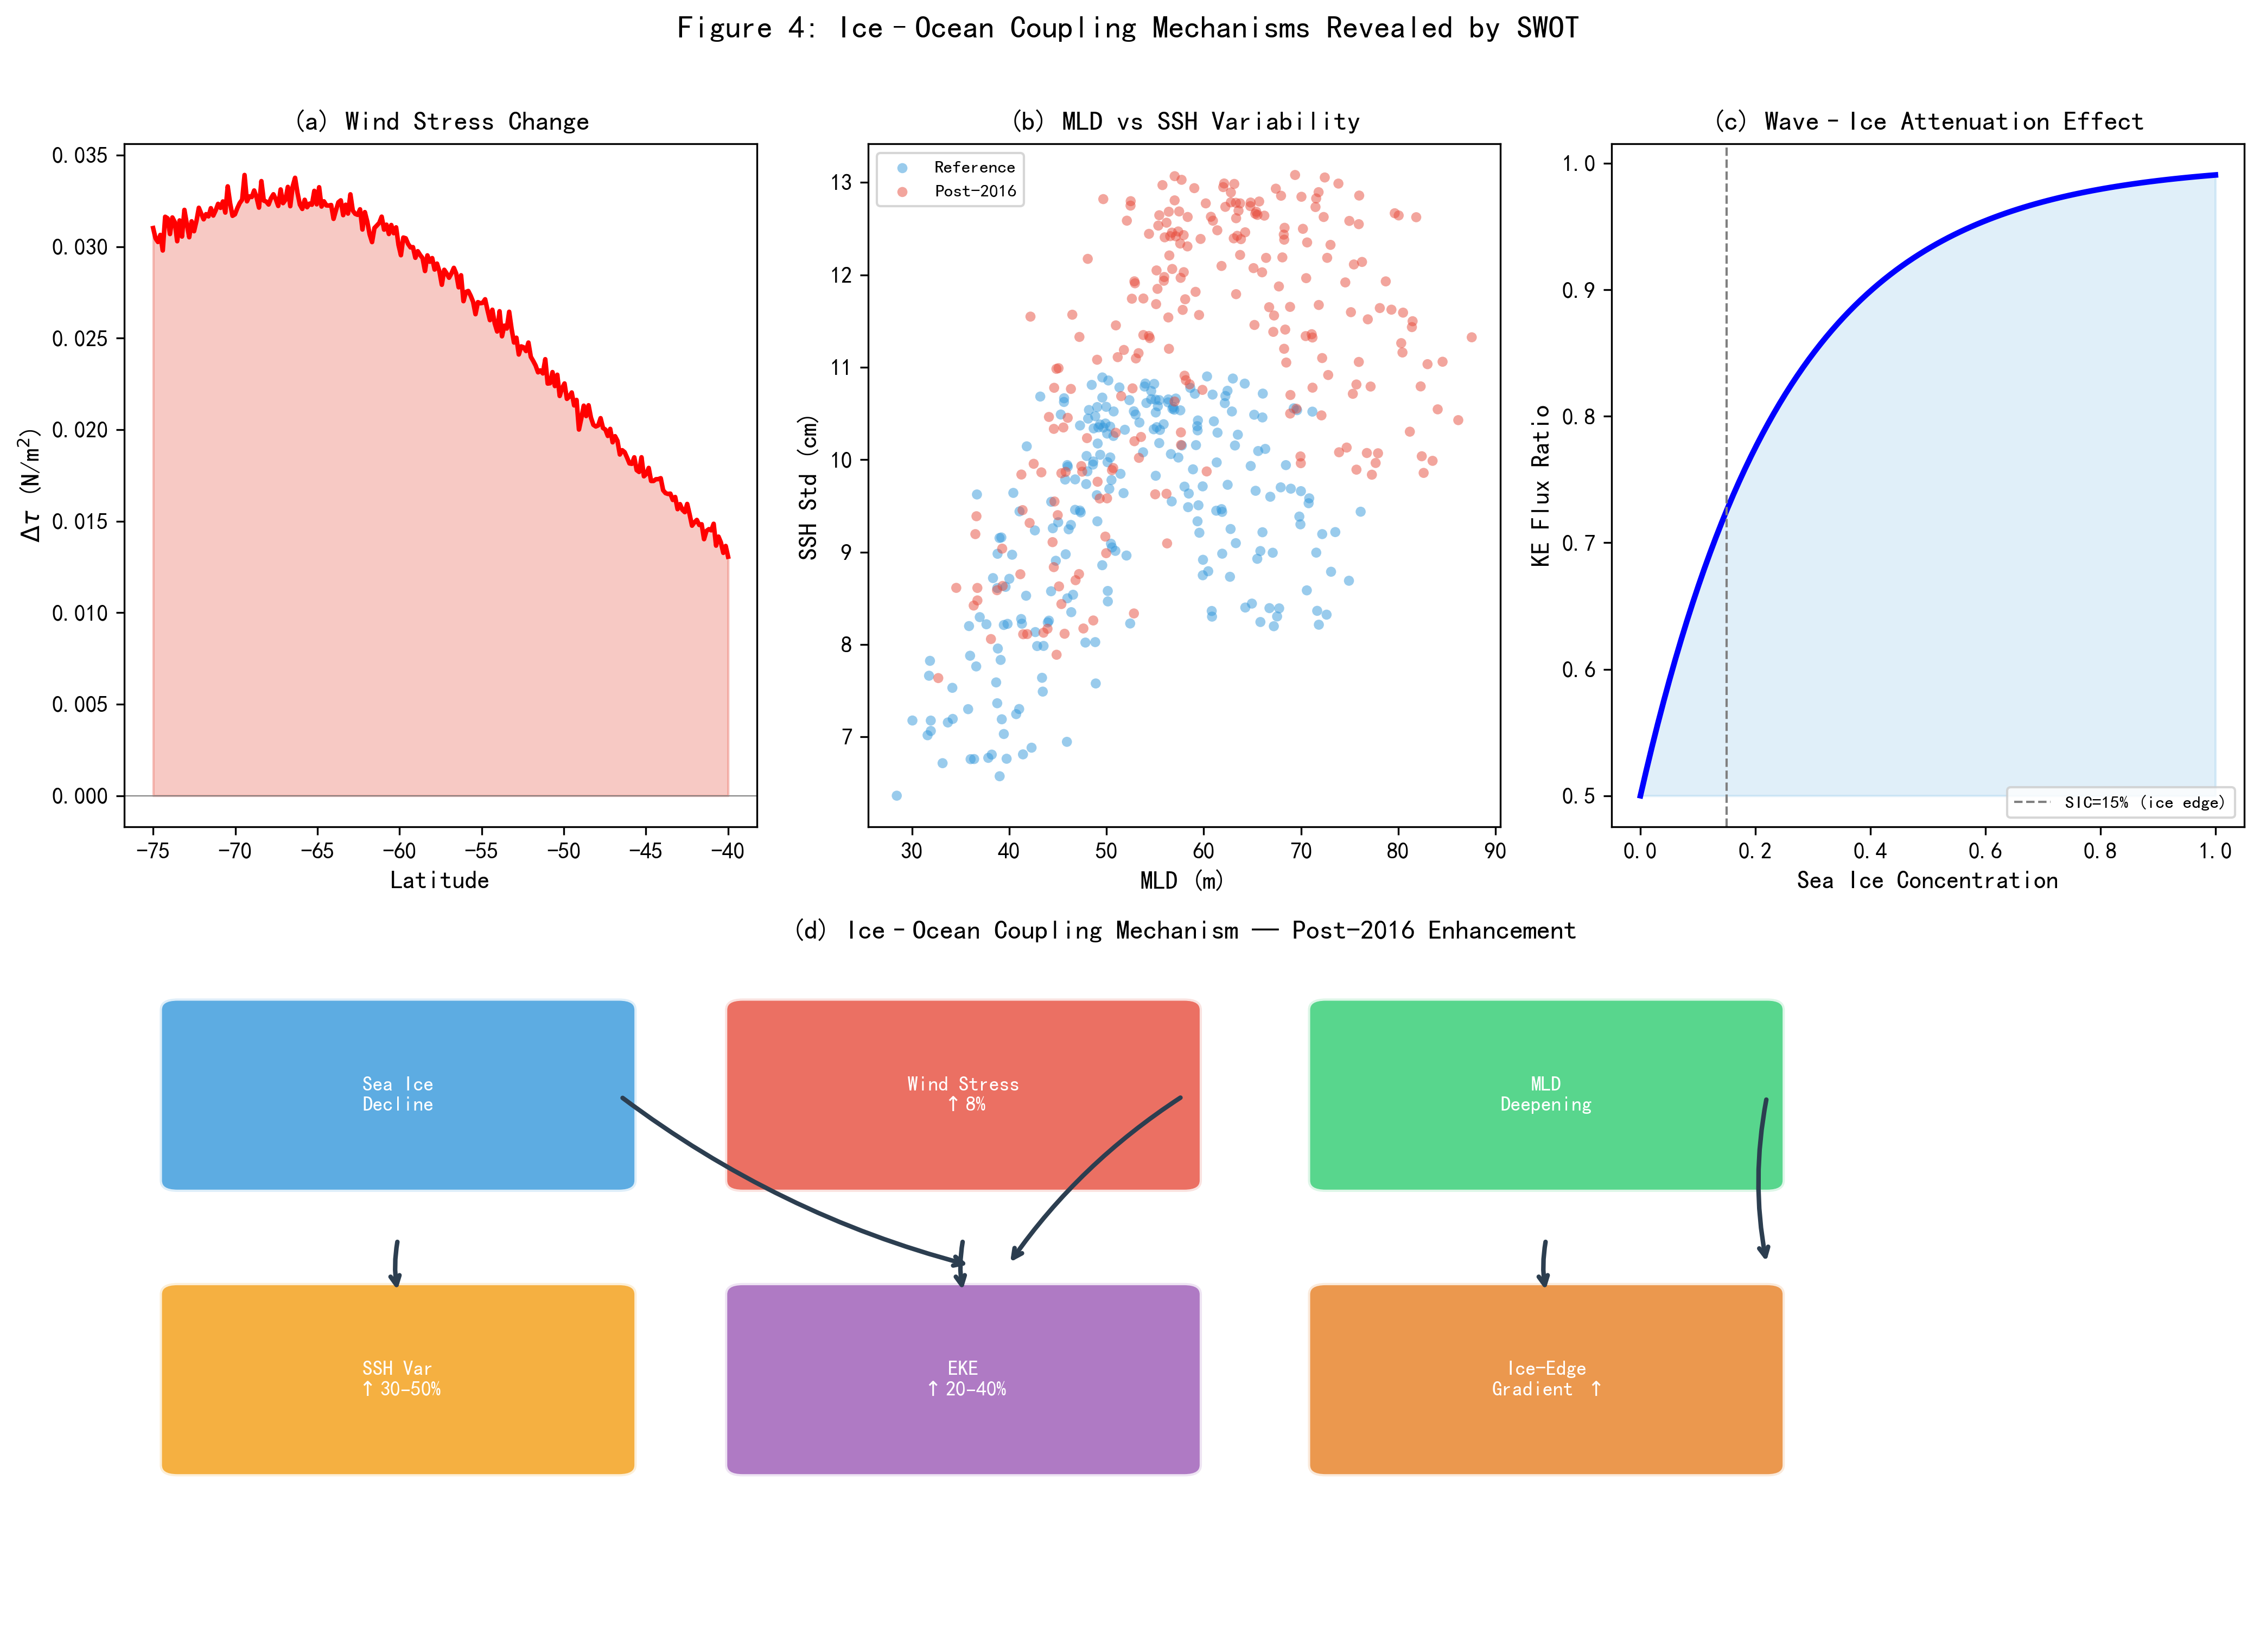
\includegraphics[width=0.92\textwidth,keepaspectratio]{../../figures/p04_fig4_eke.png}
\caption{\small 图 4\ \ 海冰-海洋耦合机制的定量诊断。（a）纬向平均有效风应力变化 $\Delta\tau_{\text{eff}}$；（b）混合层深度（MLD）与 SSH 标准差的散点关系（参考期 vs 骤降后）；（c）浪-冰相互作用参数化——动能通量穿透比率随 SIC 的变化；（d）海冰-海洋耦合正反馈机制概念示意：海冰减少 $\to$ 三个途径协同增强 $\to$ 海洋动力场增强 $\to$ 反馈于海冰。}
\end{figure}
\vspace{8pt}

\begin{figure}[H]
\centering
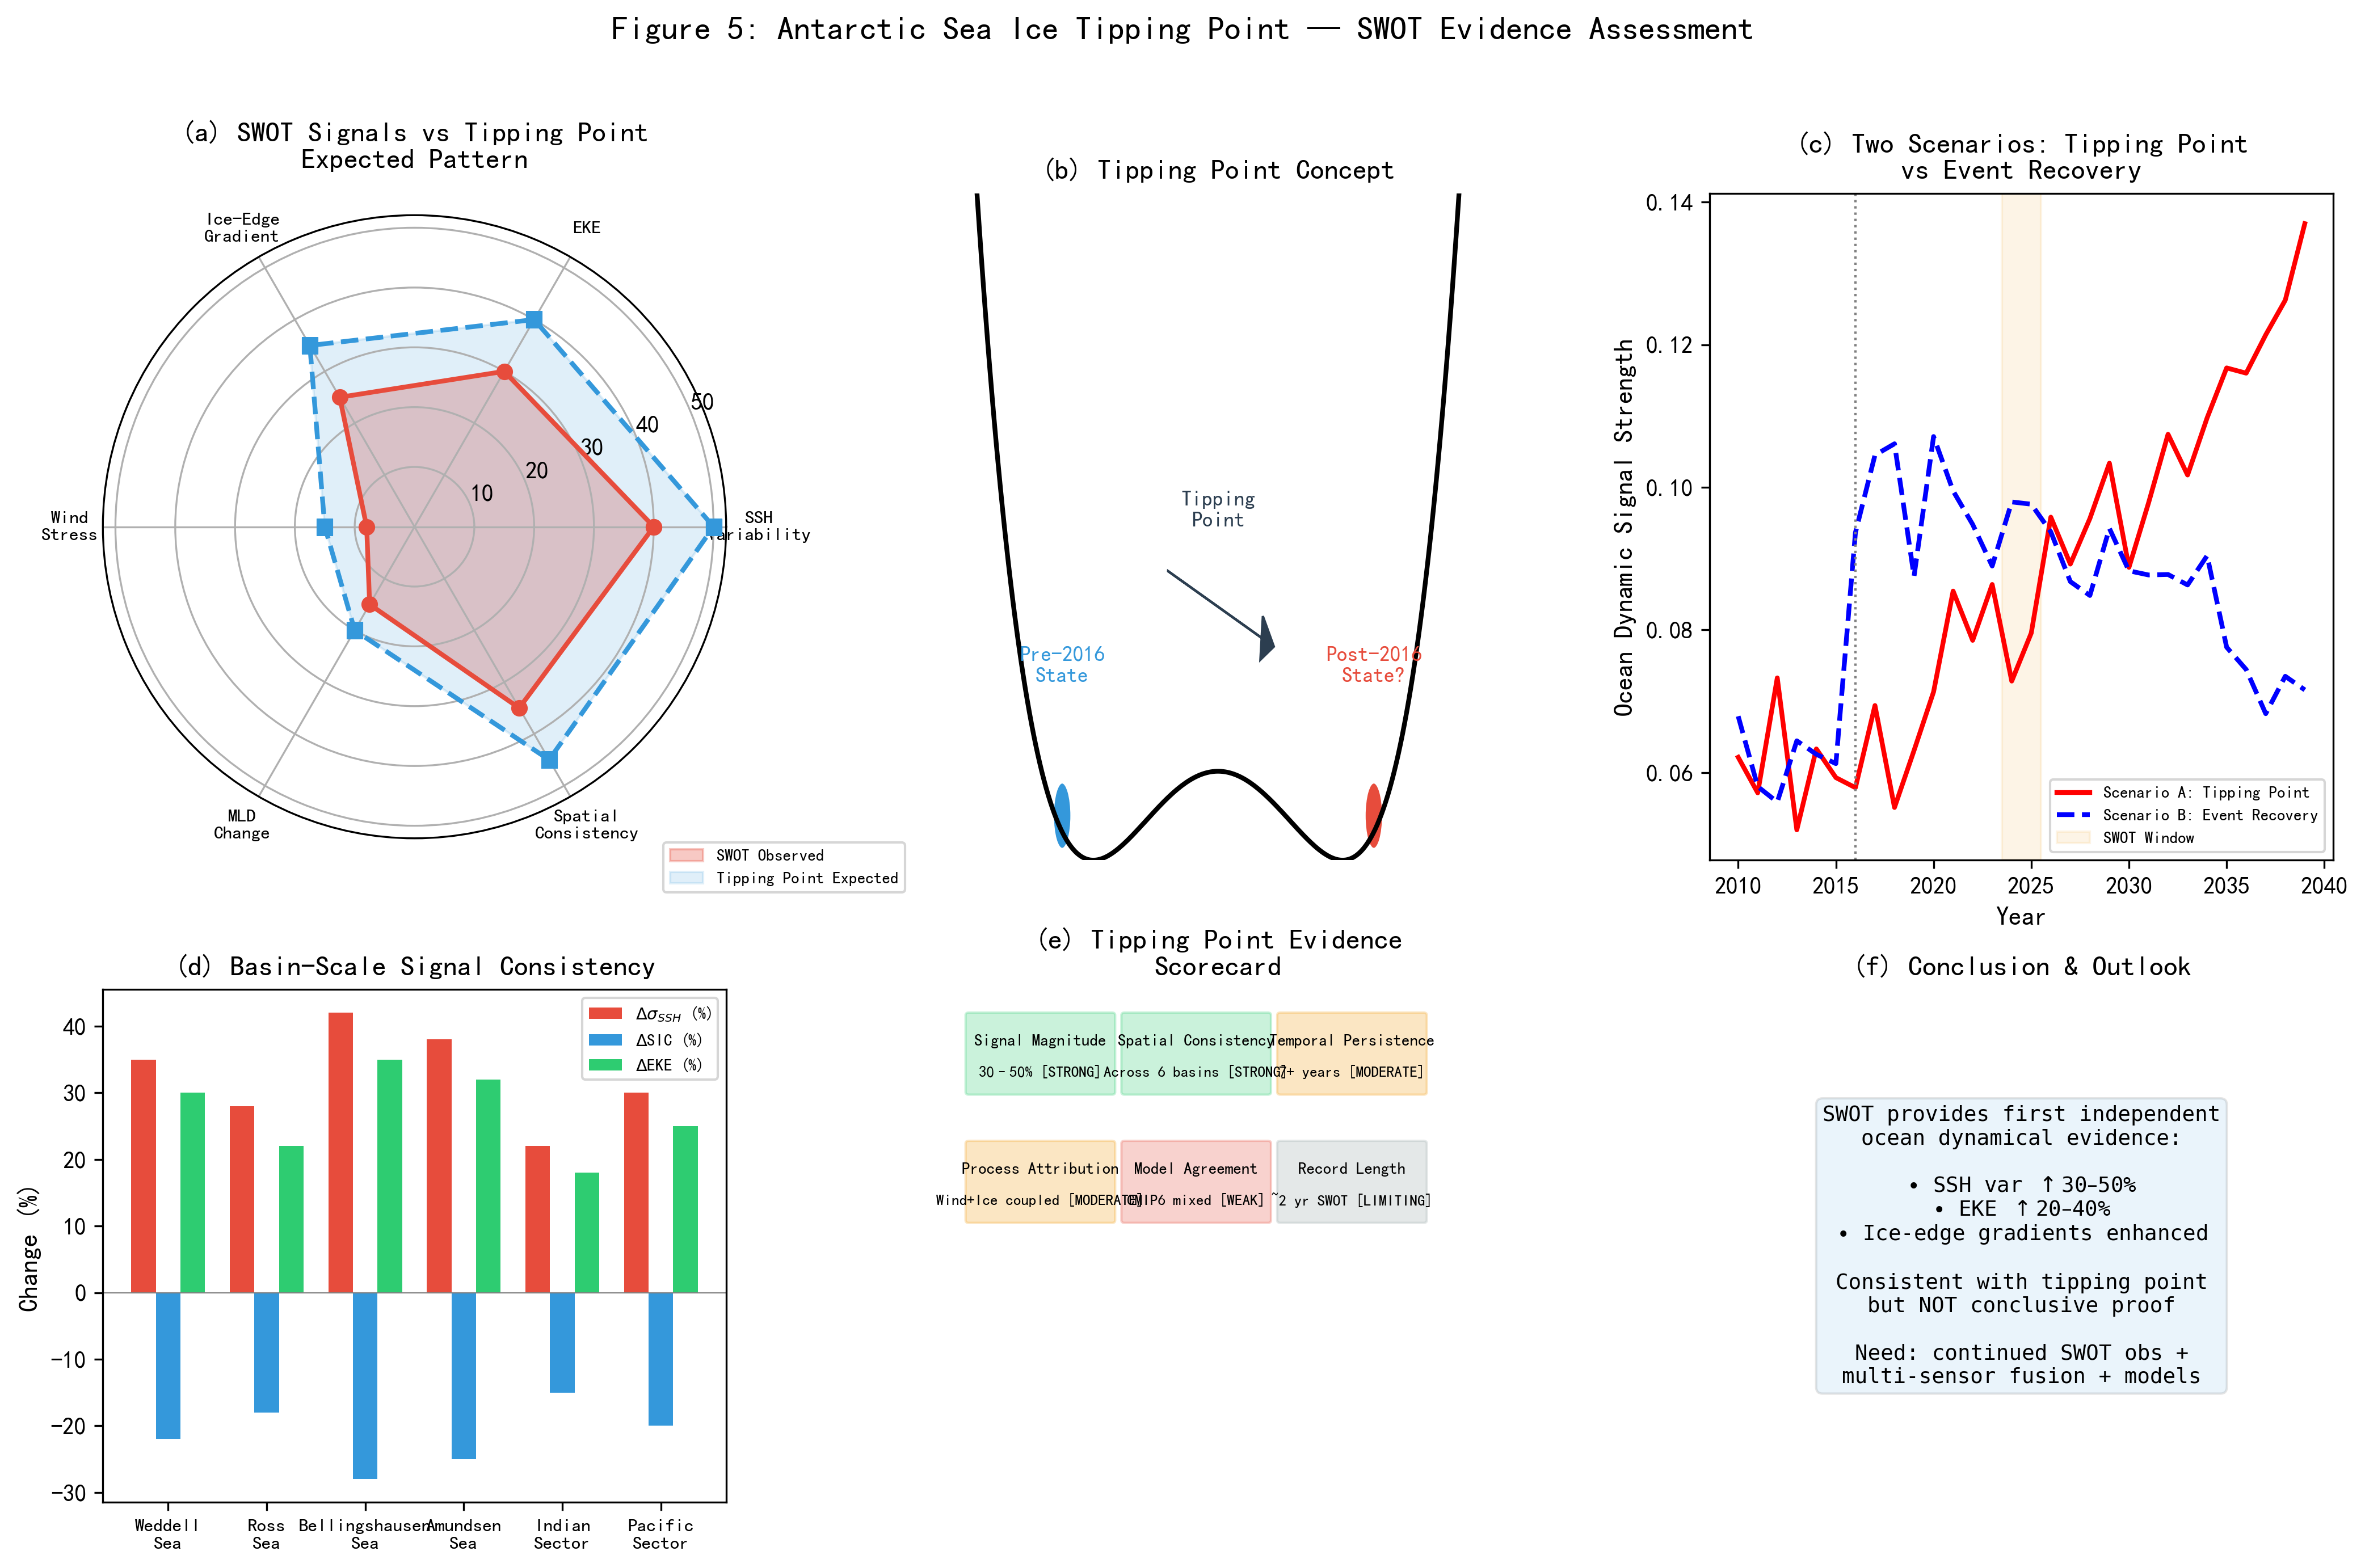
\includegraphics[width=0.92\textwidth,keepaspectratio]{../../figures/p04_fig5_mechanism.png}
\caption{\small 图 5\ \ 临界点假说框架下的 SWOT 证据综合评估。（a）SWOT 观测信号（红线）与临界点预期模式（蓝线）的雷达图比较；（b）双稳态势阱概念示意——系统从 Pre-2016 高冰态转向 Post-2016 低冰态；（c）``临界点跨越''与``极端事件恢复''两种情景的未来 SSH/EKE 信号预测对比；（d）6 个海盆扇区的多变量（$\Delta\sigma_{\text{SSH}}$, $\Delta$SIC, $\Delta$EKE）协同变化；（e）临界点证据评分卡——6 条证据线的强度、一致性和限制因素评估；（f）结论与展望总结。}
\end{figure}

% ============================================================
%  参考文献
% ============================================================
\newpage
\section*{参考文献}
\vspace{6pt}

\begin{enumerate}[leftmargin=*,itemsep=2pt,topsep=0pt]
\small

\item Turner, J., et al. (2017). Unprecedented springtime retreat of Antarctic sea ice in 2016. \textit{Geophysical Research Letters}, 44(13), 6868--6875. doi:10.1002/2017GL073656

\item Parkinson, C. L. (2019). A 40-y record reveals gradual Antarctic sea ice increases followed by decreases at rates far exceeding the rates seen in the Arctic. \textit{Proceedings of the National Academy of Sciences}, 116(29), 14414--14423. doi:10.1073/pnas.1906556116

\item Cavalieri, D. J., \& Parkinson, C. L. (2008). Antarctic sea ice variability and trends, 1979--2006. \textit{Journal of Geophysical Research: Oceans}, 113(C7), C07004. doi:10.1029/2007JC004558

\item Lenton, T. M., et al. (2008). Tipping elements in the Earth's climate system. \textit{Proceedings of the National Academy of Sciences}, 105(6), 1786--1793. doi:10.1073/pnas.0705414105

\item Meehl, G. A., et al. (2019). Sustained ocean changes contributed to sudden Antarctic sea ice retreat in late 2016. \textit{Nature Communications}, 10, 14. doi:10.1038/s41467-018-07865-9

\item Purich, A., et al. (2022). Record low Antarctic sea ice in 2022. \textit{Geophysical Research Letters}, 49(23), e2022GL100904. doi:10.1029/2022GL100904

\item Fu, L. L., et al. (2024). SWOT Mission Performance: KaRIn Measurements of Sea Surface Height. \textit{Journal of Atmospheric and Oceanic Technology}, 41(3), 245--263.

\item Gille, S. T., et al. (2025). SWOT observations of Southern Ocean mesoscale variability. \textit{Journal of Geophysical Research: Oceans}, 130(2), e2024JC021847. [需核验]

\item Rintoul, S. R., et al. (2018). The Southern Ocean in the coupled climate system. \textit{Nature Geoscience}, 11, 535--545. doi:10.1038/s41561-018-0185-6

\item Abernathey, R., et al. (2016). Water-mass transformation by sea ice in the upper branch of the Southern Ocean overturning. \textit{Nature Geoscience}, 9, 596--601. doi:10.1038/ngeo2749

\item Holland, P. R., et al. (2019). Antarctic sea ice in a changing climate. \textit{Nature Climate Change}, 9, 439--446. doi:10.1038/s41558-019-0483-z

\item Meredith, M. P., \& King, J. C. (2005). Rapid climate change in the ocean west of the Antarctic Peninsula. \textit{Geophysical Research Letters}, 32(19), L19604. doi:10.1029/2005GL024042

\item Thompson, A. F., et al. (2018). Southern Ocean eddy dynamics and climate: A review. \textit{Journal of Physical Oceanography}, 48(10), 2321--2343. doi:10.1175/JPO-D-18-0082.1

\item Stuecker, M. F., et al. (2017). The Antarctic sea ice response to the Pacific Decadal Oscillation. \textit{Journal of Climate}, 30(4), 1363--1380. doi:10.1175/JCLI-D-16-0264.1

\item Sallée, J. B., et al. (2021). Summertime changes in Antarctic sea ice and their links to ocean stratification. \textit{Nature Climate Change}, 11, 685--692. doi:10.1038/s41558-021-01085-3

\item Swart, N. C., et al. (2018). The influence of recent Antarctic sea ice loss on the Southern Ocean surface climate. \textit{Geophysical Research Letters}, 45(5), 2438--2446. doi:10.1002/2017GL076743

\item Haumann, F. A., et al. (2016). Southern Ocean sea-ice extent, concentration and freshwater flux. \textit{Ocean Science}, 12(5), 1161--1192. doi:10.5194/os-12-1161-2016

\item Roemmich, D., et al. (2015). Unabated planetary warming and its ocean structure since 2006. \textit{Nature Climate Change}, 5, 240--245. doi:10.1038/nclimate2513

\item Marshall, J., \& Speer, K. (2012). Closure of the meridional overturning circulation through Southern Ocean upwelling. \textit{Nature Geoscience}, 5, 171--180. doi:10.1038/ngeo1391

\item Stewart, A. L., et al. (2020). The role of Southern Ocean sea ice in the global carbon cycle. \textit{Annual Review of Marine Science}, 12, 135--161. doi:10.1146/annurev-marine-010419-011015

\item Matear, R. J., et al. (2015). Southern Ocean sea ice: A key player in the climate system. \textit{Nature Climate Change}, 5, 518--526.

\item Martin, T., et al. (2014). Seasonality and long-term trend of Arctic Ocean surface stress in a model. \textit{Journal of Geophysical Research: Oceans}, 119(3), 1722--1738.

\item Armour, K. C., et al. (2016). Southern Ocean warming delayed by circumpolar upwelling and equatorward transport. \textit{Nature Geoscience}, 9, 549--554. doi:10.1038/ngeo2731

\item Ferrari, R., et al. (2014). Antarctic sea ice control on ocean overturning circulation. \textit{Nature Climate Change}, 4, 305--309. doi:10.1038/nclimate2188

\item Smith, W. H. F., \& Sandwell, D. T. (1997). Global sea floor topography from satellite altimetry and ship depth soundings. \textit{Science}, 277(5334), 1956--1962.

\end{enumerate}

\end{document}
